\documentclass[11pt,oneside,letterpaper,showtrims,article]{memoir}
%\setlrmargins{0.25in}{*}{*}
%\setulmargins{0.25in}{*}{*}

\usepackage{graphicx}
\usepackage{listings}
\usepackage{verbdef}
\usepackage{xcolor}
\usepackage{xspace}
\usepackage{fancyvrb}
\usepackage{hyperref}

\usepackage{makeidx}
\makeindex

\makepagestyle{index}
\makeheadrule{index}{\textwidth}{\normalrulethickness}
\makeevenhead{index}{\rightmark}{}{\leftmark}
\makeoddhead{index}{\rightmark}{}{\leftmark}
\makeevenfoot{index}{\thepage}{}{}
\makeoddfoot{index}{}{}{\thepage}

\makechapterstyle{section}{%
  \renewcommand*{\printchaptername}{}
  \renewcommand*{\chapternamenum}{}
  \renewcommand*{\chapnumfont}{\chaptitlefont}
  \renewcommand*{\printchapternum}{\chapnumfont \thechapter\space}
  \renewcommand*{\afterchapternum}{}
}

\newcommand{\code}[1]{\texttt{#1}}
\newcommand{\var}[1]{\texttt{#1}}
\newcommand{\strong}[1]{{\bfseries #1}}

% Prints the month name (e.g., January) and the year (e.g., 2008)
\newcommand{\monthyear}{%
  \ifcase\month\or January\or February\or March\or April\or May\or June\or
  July\or August\or September\or October\or November\or
  December\fi\space\number\year
}

\newcommand{\smallcaps}[1]{\smallcapsspacing{\MakeTextLowercase{#1}}}

\newcommand{\TODO}{\textcolor{red}{\bfseries TODO!}\xspace}
\newcommand{\ie}{\textit{i.\hairsp{}e.}\xspace}
\newcommand{\eg}{\textit{e.\hairsp{}g.}\xspace}
\newcommand{\na}{\quad--}% used in tables for N/A cells


\title{High Level Applications (User Guide)}
% subtitle Tools for Accelerator Commissioning and Physics
\author{Guobao Shen, shengb@bnl.gov, Lingyun Yang lyyang@bnl.gov}
\chapterstyle{section}

\begin{document}
\begin{titlingpage}
{\begingroup% Story of Writing
\raggedleft
\vspace*{\baselineskip}
{\Huge\itshape User Guide} \\
\vspace*{\baselineskip}{\Huge\itshape of High Level Applications}\\[\baselineskip]
{\large\itshape NSLS-II commissioing tools}\\[0.2\textheight]
{\Large Guobao Shen\\Lingyun Yang}\par
\vfill
\flushleft
{\sffamily
  Schedule:\hfill
\begin{itemize}
\item 12/01/2011--02/29/2012, LINAC front end
\item 03/30/2012--07/28/2012, LINAC
\item 05/29/2012--06/28/2012, LBTL in LINAC
\item 07/28/2012--08/27/2012, LBTL
\item 08/27/2012--12/25/2012, Booster
\item 12/15/2012--01/14/2013, BSTL in Booster tunnel
\item 01/14/2013--01/24/2013, BSTL
\item 01/24/2013--09/21/2013, Storage Ring Commissioning Part 1
\item 09/21/2013--11/20/2013, ID installation
\item 11/20/2013--02/18/2014, Storage Ring Commissioning Part 2
\end{itemize}
}
\vspace*{5ex}
%{\Large \plogo{} \sffamily The Publisher}
{\small\scshape September 27, 2010}
\vspace*{\baselineskip}
\endgroup}
\end{titlingpage}


\newpage
~\vfill
\thispagestyle{empty}
\setlength{\parindent}{0pt}
\setlength{\parskip}{\baselineskip}
Copyright \copyright\ %\the\year\ \thanklessauthor

\par\textit{First printing, \monthyear}

This manual is for tools for accelerator commissioning and physics. It
is original for NSLS-II (National Synchrotron Light Source II)
project, which is under construction at Brookhaven National
Laboratory. 

Copyright @copyright{} 2010 The NSLS-II Project.


\newpage
\thispagestyle{empty}
\setcounter{tocdepth}{3}
\tableofcontents*


\chapter{Introduction}

This manual describes high level applications~(HLA\index{hla}) for NSLS-II
commissioning and accelerator physics study.

The HLA includes a set of applications and the APIs those applications are
based-on. The applications is either a simple command or an application
with graphical user interface~(GUI\index{gui}). APIs are designed for
interactive control or batch scripting. Both applications and APIs are in
a high level form that are friendly to physicists and operators.

This manual is compiled based on the requirements from the following
documents:
\begin{itemize}
\item 2008, NSLS-II: Model Based Control - A Use Case Approach~\cite{bengtsson_2008_nsls-ii}
\item 2009, Assumptions on NSLS-II Accelerator Commissioning~\cite{willeke_2009_assumptions}
\item 2010, The Path to Accelerator Commissioning~\cite{willeke_2010_path}
\item 2010, NSLS-II Storage Ring Commissioning~\cite{krinsky_2010_nsls-ii}
\end{itemize}

The details of each API can be found in the reference manual distributed
with the source code. A less detailed list of APIs is in
another manual by same authors~\cite{shen_hla_apis}.

\section{Schedule for Beam Commissioning}

\vspace{5ex}
\begin{itemize}
\item 12/01/2011--02/29/2012, LINAC front end commissioning
\item 03/30/2012--07/28/2012, LINAC commissioning
\item 05/29/2012--06/28/2012, LBTL in LINAC commissioning
\item 07/28/2012--08/27/2012, LBTL commissioning
\item 08/27/2012--12/25/2012, Booster commissioning
\item 12/15/2012--01/14/2013, BSTL in booster tunnel
\item 01/14/2013--01/24/2013, BSTL
\item 01/24/2013--09/21/2013, Storage Ring Commissioning Part 1
\item 09/21/2013--11/20/2013, ID installation
\item 11/20/2013--02/18/2014, Storage Ring Commissioning Part 2
\end{itemize}

\section{Overview of Control Scripts and Applications}

The high level control software is developed for the beam commissioning
and accelerator physics study. It is designed for monitoring, control and modeling
the electron beam and accelerators.

A set of existing tools such as MATLAB Middle Layer~(MML) will be
installed in the control room. However, more new tools need to be
developed especially for the first turn beam monitoring and manipulations.

The new developement will be based on Python language,
integrated with libraries for numerical analysis, data input/output, image
processing, network, visualization, statistics and EPICS channel access. This
environment will have both interactive control terminal and batch~(script)
processing mode. High level applications and application programming
interface~(API) will be developed to make beam manipulation and hardware
control friendly to physicists and operators.

The new Python based package will have certain overlap with MML, and will
have better integration with the global database, where all related
information are stored: from magnet bentchmark data to user profile.

This work is done by both controls group and accelerator physics group.

\section{HLA Architecture}


The system architecture is shown in Fig.~\ref{fig:arch}:

\begin{figure}
  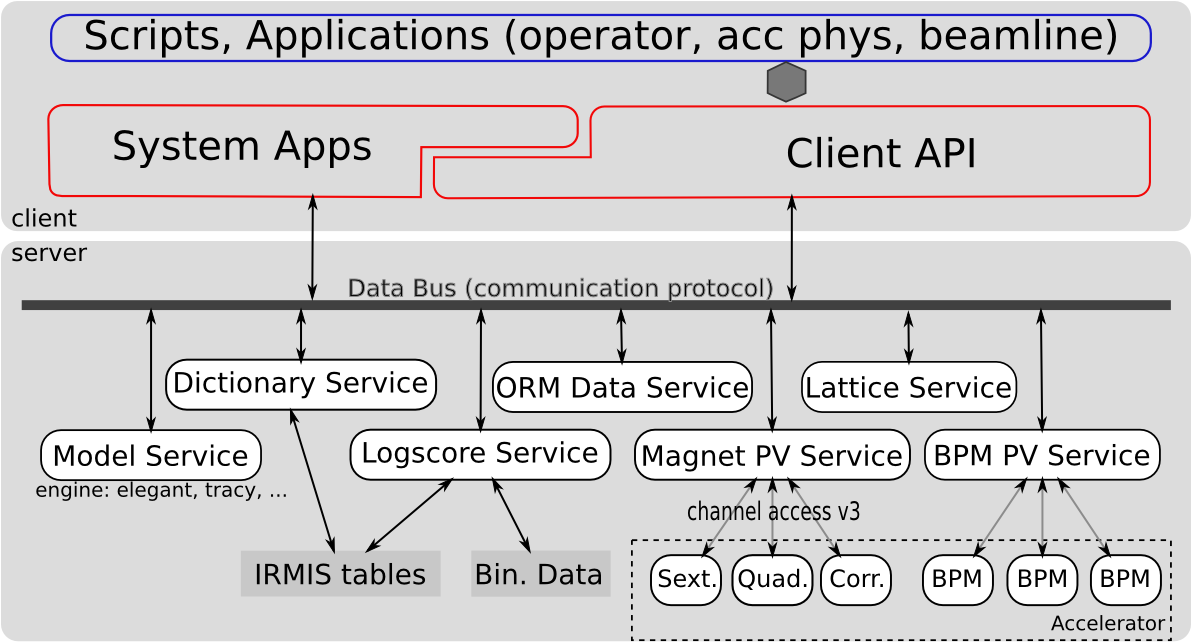
\includegraphics[width=\textwidth]{hla_arch}
  \caption{\label{fig:arch}A client/cerver based architecture for HLA}
\end{figure}

It adopts a client/server model, and consists of various servers for data
acquisition, analysis, management and communication. Based on this
structure, physics applications can be developed to satisfy the
requirements of both day-1 beam commissioning, future beam study, and
daily operation.  Briefly, the system consists of
\begin{itemize}
\item data source layer, which can be low level hardware control system,
  or a relational database;
\item a service layer, which provides services to gather data from the
  data source layer, and perform data manipulations such as constructing
  an orbit using BPM data;
\item a presentation layer, which present machine status to operators, and
  provides an interface for machine control
\end{itemize}

The server part talks directly with hardware using EPICS PV. It is an area
controls group focus on. All the data on ``data bus'' have a meaningful
name instead of long abstract channel name. e.g. the setpoint of
horizontal orbit corrector in cell 1 girder 3 is presented to accelerator
physicists as \code{CH1[0]} instead of \code{``SR:C01-MG:G03A.SP''}. This
makes them to write high level control scripts easier. The client API
which encapsulate low level control details are listed in
~\cite{shen_hla_apis}. They usually contains physics logic or accelerator
dependent quantities inside. e.g. \code{getChannelVariance},
\code{measureChromaticity}.

\begin{itemize}
\item BBA and LOCO are HLA applications. Turn by turn beam orbit
  measurement and analysis can be a HLA script.
\item Client APIs are a group of physics logics, e.g. \code{measOrbitRm},
  \code{measChromaticity}, \code{getGoldenOrbit}, ...
\item Server APIs are called by client APIs across the network, and will
  not be seen by HLA applications or scripts. The server APIs have two
  major functions:
  \begin{itemize}%[\bfseries\textenddash]
  \item manage the accelerator magnets/lattice information, e.g. logic
    group of a magnet, whether it is used by BBA or LOCO or orbit
    measurement etc. The basic information is contained in a XML file or a
    database in the following sections, (the implementation may not be a
    XML file, but a Database). lattice layout. (optional: nearby vacuum
    and temperator sensor information, power supply name and location)
  \item control the magnets via a control server, this server will call
    low level APIs to do PV readings and settings.
  \end{itemize}
\end{itemize}

The high level applications developed by accelerator physicists should
be able to achieve their goals by focusing on algorithms while being
released from tedious data acquisition and manipulation issues. This
is the design strategy for the software architecture. With a clean and
carefully designed interface, collaborators, who have different areas
of expertise such as GUI design, numerical analysis, accelerator
physics, data acquisition, hardware control, and so on, can work
together effectively and productively.

\chapter{Software Requirement}

This chapter describes software requirement for NSLS-II
commissioning. This list is mainly from \cite{willeke_2009_assumptions}
and \cite{krinsky_2010_nsls-ii}, plus some personal experiences.

The items marked with (*) will get more focus, since they usually contains
more physics or algorithm. Parameters tuning or even new algorithms may be
needed. A more detailed list specfically for accelerator physics related
functions are in Chapter~\ref{chap:aptoolkit}.

Chapter~\ref{chap:apps} and Chapter~\ref{chap:aptoolkit} will give
applications and scripts to meet the following requirements.

\section{General Operation}

\begin{itemize}
\item Overall status page (warning when read/set are different too much ?)
\item Status, Alarm and warning monitor
\item Permit system monitor and control
\item Data logger and data display
\item Electronic logbook
\end{itemize}

\section{Operations Software}

\begin{itemize}
\item Accelerator parameter store/restore (*)
      \begin{enumerate}
      \item manage, editing capability for stored accelerator status.
      \item smoothly ramp from one stage to another.
      \item compare two stages, online and saved data, two data file.
      \end{enumerate}
\item Injection Control
\item Power supply control
\item RF control
\item Fast orbit feedback control
\item Front-end monitoring and control
\item Machine protection system display and control
\item Magnet temperature interlock display and control
\item Scraper and movable mask operations
\end{itemize}


\section{Major Subsystem Control}

\begin{itemize}
\item Power supply page which lists for all PS:
      \begin{enumerate}
      \item setting or waveform, read back
      \item difference between DCCTs, status
      \item recent history.
      \end{enumerate}
\item RF page with all relevant settings, read back, status, parameters
\item Vacuum display and control. ``Water flow'' or 3D plot of vacuum status along the ring with time line info.
\item Cryogenics system display and control
\item Pulsed magnet systems monitor and control
\end{itemize}


\section{Beam Diagnostics}

\begin{itemize}
\item Beam orbit page with closed orbit, turn by turn, single turn, status
  information, difference (referecne orbit display) (*)
\item Beam current history and lifetime display (*)
\item Bunch intensity display and history display/analysis (*)
\item Beam emittance display (*)
\item Injection element display and control page (*)
\item Injection efficiency
\item Timing system display and control 
\item Synchronization system display and control
\item Tune display and control (*)
\item Temperature monitoring display
\item Bunch length and profile if it is available (*)
\item Measure BPM linearity
\end{itemize}

\section{Safety Systems}

\begin{itemize}
\item Personal protection system status display
\item Equipment protection status display and control
\item Beam containment status display and control
\item Top-off status monitor
\end{itemize}

\section{Utility Control}

\begin{itemize}
\item Tunnel air temperature and humidity monitor
\item Mechanical utilities status and controls
\item Electrical utilities status and controls
\item Equipment enclosure monitor
\item Water colling system display
\item Controls network monitor
\end{itemize}


\section{Beam Status Diagnostics}

A set of API should be provided to allow physicists to fetch data from
circular buffer of related sub-system, especially diagnostic
instrument, and RF. Detailed requirement can be found in~\cite{shen_cbd}.



\chapter{High Level Applications\label{chap:apps}}

The HLA and Controls are divided into three layers: HLA applictions and
scripts, client APIs and server API~(\cite{shen_hla_apis}).  The users
(accelerator physicists, operators and beamline scientists) will normally
access the first two forms: use applications/scripts by mouse clicks, and
the APIs in an interactive command line.


Applications include:
\begin{itemize}
\item Overall status of all subsystems: magnet, vacuum, RF, temparature
\item Orbit display and correction.
\item Linear optics reconstruct, i.e. LOCO
\item Beam based alignment.
\end{itemize}

APIs are defined in \cite{shen_hla_apis}, and are used by HLA
applications. They include data acquisition, processing and storage, and
can be combined for different purpose. The APIs are in Python language,
and can be used in both interactive environment or scripts. Necessary
packages including linear algebra, frequency analysis, statistics, data
IO, database, network, regular expression and visualization will be
provided. See \cite{python} (\url{http://www.python.org}), \cite{scipy}
(\url{http://www.scipy.org}), \cite{numpy}
(\url{http://numpy.scipy.org/}, \cite{ipython}
(\url{http://ipython.scipy.org/}), \cite{matplotlib}
(\url{http://matplotlib.sourceforge.net/}).


The HLA applications are those have a stable algorithm and data
flow. Each is in a standalone form.


\section{Machine Status}

The applications will provide overall status of the whole machine, and
give warnings when any abnormal beam behaviour is detected, for example
a readback differs from setting point larger than its threshhold. The
status includes beam information, and hardware status including magnet
and its power supply, vacuum, RF, and so on.

These part can be done in striptool, EDM or CSS (control system
studio). No heavy data manipulation or physics logics. 

% \TODO Can CSS/EDM do simple caput ? I think yes.

\begin{itemize}
\item Tunes
  \begin{itemize}
  \item horizontal/vertical tune number, at least 1Hz update
  \item optional: FFT of turn by turn BPM data, choice of any live BPM.
  \item optional: 2D tune footprint with resonance lines
  \end{itemize}
\item Magnets, tables of data. SP/RB of main magnets: quadrupoles, sextupoles, correctors.
\item Vacuum status in plots and tables.
  \begin{itemize}
  \item Pressure vs index.
  \item optional: Pressure vs pump location.
  \item optional: waterflow plot.
  \end{itemize}
\item RF status
  \begin{itemize}%[\bfseries\textenddash]
  \item optional: RF feedback status which detects orbit drift vs RF frequency.
  \end{itemize}
\item Feedback status
\item Beam profile: current, size, rms, center, image.
\end{itemize}


\subsection{Orbit Display and Correction}

This application displays and controls electron orbit.
  
\begin{itemize}
\item Static orbit display
  \begin{itemize}%[\bfseries\textenddash]
  \item Plot static orbit. (with magnet layout)
  \item Show golden orbit (or reference orbit)
  \item Absolute orbit offset and orbit offset with respect to golden orbit
  \item Plot orbit change from now on.
  \item Orbit statistics. stability, especially drift and variation
  \end{itemize}
\item Static orbit control
  \begin{itemize}%[\bfseries\textenddash]
  \item Correct static orbit with selected correctors and BPMs
  \item Enable/disable BPMs for orbit correction and feedback.
  \item Enable/disable correctors for orbit correction and feedback
  \item Import/export orbit response matrix
  \item Edit golden orbit offset. (e.g. offset the golden orbit to create local bump)
  \end{itemize}
\item Orbit feedback status
\item Turn by turn BPM
  \begin{itemize}%[\bfseries\textenddash]
  \item reading vistualization when available/enabled
  \item get/plot turn-by-turn BPM signal, including orbit and sub/diff
  \item Realtime tune based on turn-by-turn BPM
  \item BPM buttons readout.
  \item plot single shot orbit.
  \item Correct orbit based on single shot orbit
  \end{itemize}
\item Measure the orbit response matrix, with flexible number of BPMs
  and correctors.
\end{itemize}

Bad BPM identification should be done in other application. Data
synchronization to be done in low level server part.

Interplay with feedback system when creating local bump: update the
reference orbit to feedback ? or share same orbit difference from a
dedicated IOC ? the feedback should check golden orbit at 10-50Hz rate
if real-time orbit difference is not available to it.


\subsection{Beam Based Alignment (BBA)}

BBA use a list of correctors, BPMs and nearby quadrupoles, to steer the
beam through center of these quadrupoles. The input is a list of
corrector-BPM-quadrupole triplets.  The BPMs in corrector-BPM-quadrupole
triplet is a subset of live BPM.  This needs to get the golden orbit,
set the golden orbit, line fitting, step the quadrupole, step the
corrector (this can be a ``macro step'', e.g. 10 times than normal step
size). Many raw data needs to be saved in certain format: Python binary, HDF5 or Matlab.

We would prefer to have all data saved, corrector settings/readings, BPM
readings and Quadrupole settings/readings.

The measurement and analysis can be separated conceptually, which makes
the post processing< easier, i.e. we can analyze any historical data,
and replay them.

It should work on separate set of quadrupoles, and combine data with previous measurement.

\subsection{Linear Lattice Fitting (LOCO)}

\begin{itemize}%[\bfseries\textenddash]
\item analyze quadrupole gradient error.
\item analyze BPM gain error.
\end{itemize}

It requires:
\begin{enumerate}
\item Designed orbit response matrix (ROM)
\item change specified correctors 
\item get closed orbit change at specified BPM
\end{enumerate}

This application needs mathematical package to do minimization and
singular value decomposition (SVD). It also requires simulator for
fitting.

\subsection{Measure TWISS Parameters}

\begin{itemize}%[\bfseries\textenddash]
\item measure beta functions
\item measure dispersion
\item measure chromaticity
\item measure coupling
\item measure coupling response matrix
\item Measure and adjust tune. (tune scan ?)
\item Measure and correct the chromaticity (linear and nonlinear). 
\item Measure beam optics including phase advance, beta functions, dispersion.
\item Dispersion measurement and correction, optimal set of quads
\end{itemize}

\subsection{Smooth Ramping}

\begin{itemize}%[\bfseries\textenddash]
\item list channels we are interested.
\item ramp whole group at certain rate.
\end{itemize}
It requires:
\begin{enumerate}
\item searching for channels (regular expression, wild-card)
\item save state/read stage.
\end{enumerate}
The control group may provide ramping for whole storage ring, here this
application can ramp specified channels between two states.

\subsection{History Analyzer}

\begin{itemize}%[\bfseries\textenddash]
\item view archive data in certain time frame.
\item link to logbook to view reasons for shutdown, current drop (?)
\item simple statistic for the data: average, variance, maximum, minimum.
\item print, save figures.
\end{itemize}


\subsection{Insertion Device Related (Matching)}

\begin{itemize}%[\bfseries\textenddash]
\item get/correct closed orbit distortion
\item get/correct phase distortion
\item get/correct coupling distortion
\end{itemize}

\subsection{Simulator}

This is required for online lattice fitting, e.g. LOCO. elegant or Tracy-II can be a choice.



\chapter{\label{chap:aptoolkit}Accelerator Physics Toolkit}

By toolkit, we mean a short script based on CAPIs. Not like HLAs, they
have small set of functions, but easy to understand and modify. For
example we put a small script \code{probeBpmStability} into this category,
since it is mainly a function call of \code{getBpmVariance} plus checking
against certain criterial.

One interactive \code{Python} environment is also provided for
interactive control of the storage ring. In this interactive
environment, a set of APIs are provided to make physicists who has no
knowledge of EPICS or low level channel access be able to do many
measurements and diagnostics.

This interactive mode can also run as batch mode, which makes the
prototyping of new HLA and algorithms easier.

The plotting features are only in interactive environment and GUI
applications. Scripts and save pictures in \code{png}, \code{jpeg},
\code{pdf} and \code{eps} format.

Since the CAPIs (client APIs) are from requirement analysis of NSLS-II
commissioning plan, we can describe those accelerator physics tasks and
the related APIs (both client and server).

\section{Requirement}

We have compiled a set of requirements for high level control software,
and design the APIs as a common library. The high level applications will
use these APIs to fulfil comissioning, operations and physics studies. We
need more input from operation group to make these tools more
operator-friendly.

In NSLS-II storage ring commissioning plan~\cite{willeke_2009_assumptions,
  krinsky_2010_nsls-ii}, we have defined the requirement of control
software. Here we only summarize the functions needed, but neglect the
order of using them in the commissioning.

\subsection{Hardware/Control checking and testing}

\begin{itemize}
\item BPM testing stability, polarity.
\item BPM current dependency, resolution.
\item Check polarity of all magnets.
\item Orbit corrector polarity and strength test, 
\item Converting between machine unit and physics unit.
\item Ramping from one magnet setting to another.
\item Monitoring stability of any readings and online data: magnet
  readback, orbit, temperature, vacuum.
\item Magnetic field measurement and modeling, determine calibration
\item Verify named devices in control system, control proper hardware
\item Complete survey of magnetic elements
\item Test diagnostic equipment without beam
\end{itemize}

\subsection{BTS transport line}

Obtain good transmission through septum and good transverse phase space
match, set timing of pulsed magnets.

\subsection{Insertion Device}

\begin{itemize}
\item When necessary compensate the linear optics for ID
\item Observe orbit and tune shift vs gap
\item Measure lifetime vs gap
\item Observe beam stability vs current
\item Measure change in impedance due to ID chamber
\item Prepare look-up tables for feed forward orbit correction coils.
\item Measure effect on tune shift with amplitude, chromaticity, and emittance coupling.
\item Measure impedance vs gap for IVUs
\item Commission undulator gap control for users
\item Measure flux and brightness
\end{itemize}

\subsection{Misc}

\begin{itemize}%[\bfseries\textenddash]
\item Test fast orbit feedback system.
\item Look for magnet errors that may have been missed in testing.
\item Obtain first turn in storage ring using single kicker
\item Use flag to obtain beam size information at injection point and
  after one turn.
\item Beam based alignment of sextupoles.
\item Develop lattice model using measured fields, linear/nonlinear optics.
\item Reduce beta beat
\item Correct coupling using skew quadrupoles, local and global.
\item Analysis on nonlinear dynamics.
\item Use pinger to measure tune shift with amplitude, dynamic aperture
  and characterize sextupole distribution
\item Wakefield modeling and tracking studies, develop model for
  impedance and wakefields, caculation and measurement, estimate
  instability thresholds, simulate bunch-by-bunch feedback with
  realistic bunches and wakefields.
\item Characterize ring impedance using beam.
\item Commission loss control minitoring system
\item Use visible synchrotron light monitor to study transverse beam
  profile and disturbance due to kickers. \code{getBeamProfile}
\item Study lifetime versus vacuum pressure, vertical beam size, scraper, dynamic aperture.
\item Commission transverse bunch-by-bunch feedback
\item Measure variation of coherent tune with current
\item Study increasing chromaticity from +2/+2 to +5/+5
\item Commission undulator gap control in control room
\item Calibration/Testing of Equipment Protection Interlock System
  \begin{itemize}%[\bfseries\textenddash]
  \item Center photon beam in exit slot
  \item Verify gap open/close status is properly reported to interlock system
  \item Measure interlock BPM offset and scale factors.
  \item Adjust the hardware trip points on the local logic chassis
  \item Verify beam is dumped at the specified position offsets.
  \item Set the values in the interlock test file
  \item Verify the proper operation of the interlock test
  \end{itemize}
\item Top-off Injection
  \begin{itemize}
  \item Check position of apertures in ring and beamline
  \item Test interlocks
  \item Characterize injection transient on transverse orbit, contribution from septum and kickers.
  \item Test transverse feedback with injection transient
  \end{itemize}
\item Concerns: accuracy of magnet calibration-two types of dipoles, magnetic field quality (IRMIS data).
\item PBPM matching. Read both BPM and PBPM, and use BPM to benchmark the
  PBPM values.
\item Get groud motion and chamber motion if there are available readings.
\item Monitor beam loss. Get loss monitor readings from beam containment
  system (beam loss monitor).
\item Identify MPS (magnet power sypply) ripples.
\end{itemize}


\subsection{Injector}

Software routines needed for the injector commissioning and operation are
listed in this section. Some of these routines will be delivered by linac
and booster vendors, others have to be developed by ourselves.

\begin{itemize}
\item Linac
\begin{itemize}
\item Diagnostics calibration
\item Routines for optimization of linac performance
\item Energy feedback
\item Charge feedback
\item Specification of bunch train format    
\item Beam loading compensation      
\item Energy measurement     
\item Energy spread measurement      
\item Emittance measurement (3 screens)      
\item Emittance measurement (quad scans)     
\item Matching of Twiss parameters into booster septum       
\item Beam stacking  
\item Beam transmission optimization 
\item TL quad centering      
\item Integration of safety devices/interlocks       
\end{itemize}

\item Booster
\begin{itemize}
\item Diagnostics calibration       
\item Orbit correction       
\item Tune measurement system
\item Energy measurement     
\item Momentum compaction measurement
\item Emittance measurements 
\item Beam stacking  
\item Extraction optimization
\item Ramp optimization      
\item LOCO-type machine characterization     
\item MIA in transport line -- booster acceptance testing
\item Orbit feedback 
\item Synchrotron Radiation diagnostics      
\item Bunch cleaning system  
\item TL quad centering      
\item Integration of safety devices/interlocks       
\end{itemize} 

\item SR

  In addition to what has been already specified by Accelerator Physics:

\begin{itemize}
\item Closed bump optimization: A and t
\item Simultaneous measurements of injected/stored beam orbits
\end{itemize}

\end{itemize}


\section{Terminology for High Level Applications}

The naming convension and terminology should follow the definitions of
project nomenclature standard:

\begin{itemize}
\item National Synchrotron Light Source II - Nomenclature Standard~\cite{lt_2009_nomenclature}
\item National Synchrotron Light Source II - Accelerator Systems
Requirements Document, Storage Ring Physics Nomenclature Standard~\cite{lt_2008_nomenclature}
\end{itemize}

A set of commonly used words are explained in the following:

\begin{enumerate}
\item \emph{Mode\index{mode}}
is used for separating different machine settings. As an example, there
could be ``production mode'', ``accelerator physics beam study mode'',
``short bunch mode'', ``low current mode''. With this separation, all
the other settings can be same or different for two modes.

\item \emph{Group}\index{group} represents a set of elements when they are
  sharing similar position, symmetry, purpose, connections or user's
  preferences. For example, we can assign all sextupoles with a group name
  \code{sextupole} and all magnets on the second girder in each cell a
  group name \code{girder2}. From lattice point of view, we can have a
  group name \code{qh1} for all quadrupoles with this symmetry. Each
  element or magnet can belong to one or more groups.  For consistancy,
  the element belongs to the group which has only himself and the group
  name is same as its element name (the element name is guaranteed
  unique).

  We can have some predefined group names, and they will be commonly used
  for their type or symmetry, e.g. \code{quadrupole}, \code{sh1}. The
  pre-defined group name should be discussed carefully, and stored in a
  relational database, \code{IRMIS} for example. Users can also define
  their own group name which should not overwrite any system defined group
  names.

  The suggested candidates of group name are:
  \begin{itemize}
  \item Magnet with same power supply or lattice symmetry.
  \item \code{bpm}, \code{corrector}, \code{quadrupole}, \code{sextupole},
    \code{skewquadrupole}, ...
  \item Specific purpose: \code{bba}, \code{orbit}, \code{tune},
    \code{chromaticity}
  \item User defined: ``Sam's test BPM'', ``Weiming's Toy'', ...
  \end{itemize}

  \index{wildcard} When searching for a group, the name matching should
  support a subset of regular expression (need more details on ``subset'',
  how small/large is this set). One choice is the BASH wildcards:
  \begin{itemize}
  \item \strong{*}, zero or more characters
  \item \strong{?}, exactly one character
  \item \strong{[abcde]}, exactly one character listed
  \item \strong{[a-e]}, exactly one character in the given range
  \item \strong{[!abcde]}, any character that is not listed
  \item \strong{[!a-e]}, any character that is not in the given range
  \item \strong{\{debian,linux\}}, exactly one entire word in the options
    given
  \end{itemize}
\item \emph{Sequence}\index{sequence} We can also use sequence to identify
  one element, usually BPM or corrector. For the convenience purpose when
  looping over BPM or correctors one after the other along the ring, we
  can use number as its order, instead of their names. Suggested sequence
  could be a pair [\emph{cell}, \emph{index}], and \emph{cell} is the cell
  number following the name convention as below, which is an integer
  between 1 and 30 according to the NSLS-II
  nomenclature~\cite{lt_2008_nomenclature,lt_2009_nomenclature}. The index
  is the order (according to s-location) in that cell, and index starts
  from 0 to follow some language conversion such as Python/C/C++. A
  definition similar to \code{MML (Matlab Middle Layer)} can be
  atopted. This part should be discuss carefully to avoid ambiguity.
  \index{coordinate} \index{original point}
\item \emph{Coordinate definition}, we always use \code{x}, \code{y} and
  \code{s} specify the horizontal, vertical and longitudinal plane. The
  $s=0$ is defined as the injection point (in Cell 30).
\item \emph{Array Data Arrangement\index{array}} Whenever the value is an
  array, sort it in the beam direction, for example, in increasing order
  of $s$ location. This may be confusing for the injection cell, where
  $s=0$ does not aligned with the begin/end point of a cell, but in the
  middle.

  A policy to determine who is the first element should be
  discussed. ($s=0$ location)

\item \emph{Control System}
\begin{enumerate}
\item EPICS\index{EPICS}
\item Channel\index{Channel}
\item Record\index{Record}
\item PV (Process Variable)\index{PV}\index{Process Variable}
\item CA (Channel Access)\index{CA}\index{Channel Access}
\end{enumerate}
\end{enumerate}





\appendix

\chapter{Acronym and API Prefix}

We recommend to use full word instead of acronym, but for the most
common ones, acronym makes life easier. The following list serves as a
guideline for API prefix but exceptions do exist.
\begin{itemize}
\item \strong{meas} is for measurement routines. They may perturb the beam, and affect users.
\item \strong{get} is either read history or the output of online instrument.
\item \strong{set} will change the settings of an online instrument. The value will be gone after next injection(non-topoff)
\item \strong{save} operates on file, read machine to file/DB. (set operates on real machine, on a smaller scale, single element/group). The new value will take effect in next injection/run. 
\item \strong{load} operates on files/DB and set to memory/machine.
\item \strong{calc} is for routines doing calculation and analysis. This is calculation only, does not perturb the beam.
\item \strong{enable/disable} makes element online/offline
\end{itemize}

There are exceptions that a few APIs have prefix not mentioned above
(see \cite{shen_hla_apis} for a complete list).

BPM(beam position monitor), RF(radio frequency), SOFB/FOFB(slow/fast
orbit feedback), bba(beam based alignment), chrom(chromaticity),
sp(setpoint), rb(readback) are common acronyms.


%
% -------------------------------
%

\begin{thebibliography}{99}
\bibitem{bengtsson_2008_nsls-ii} J. Bengtsson, B. Dalesio, T. Shaftan,
  T. Tanabe, \emph{NSLS-II: Model Based Control - A Use Case Approach},
  Tech-note 51, Oct 2008
\bibitem{willeke_2009_assumptions} F. Willeke, \emph{Assumptions on
    NSLS-II Accelerator Commissioning}, November 22, 2009
\bibitem{willeke_2010_path} F. Willeke, \emph{The Path to Accelerator
    Commissioning}, talk on ASD Project Meeting, Jan 2010
\bibitem{krinsky_2010_nsls-ii} S. Krinsky, \emph{NSLS-II Storage Ring
    Commissioning}, NSLS-II ASD Retreat, May 13, 2010.
\bibitem{lt_2009_nomenclature} \emph{National Synchrotron Light Source II
    - Nomenclature Standard}, LT-ENG-RSI-STD-002, Jan 21, 2009, Rev 2
\bibitem{lt_2008_nomenclature} \emph{National Synchrotron Light Source II
    - Accelerator Systems Requirements Document, Storage Ring Physics
    Nomenclature Standard}, RSI Document 1.3.4-001, Feb 17, 2008, Rev 1
\bibitem{shen_cbd} G.~Shen, Y.~Hu, B. Dalesio, \emph{Circular Buffer
    Diagnostic}
\bibitem{shen_hla_apis} G.~Shen, L.~Yang, \emph{High level applications -
    APIs}
\bibitem{python} Python, \url{http://www.python.org/}
\bibitem{ipython} iPython, \url{http://ipython.scipy.org/moin/}
\bibitem{matplotlib} matploblit, \url{http://matplotlib.sourceforge.net/}
\bibitem{scipy} SciPy, \url{http://www.scipy.org/}
\bibitem{numpy} SciPy, \url{http://numpy.scipy.org/}
\end{thebibliography}

%
%

\pagestyle{index}
\printindex

\end{document}
